\documentclass{standalone}
\usepackage{tikz}

\begin{document}
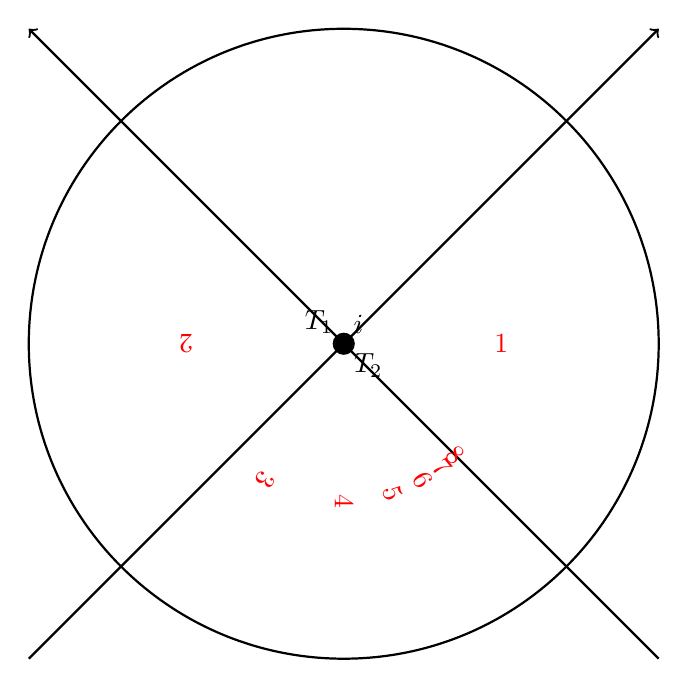
\begin{tikzpicture}[scale=2]
    % Draw the circle representing the neighborhood around the intersection point
    \draw[thick] (0,0) circle (2);
    
    % Mark the intersection point
    \fill (0,0) circle (2pt) node[above right] {$i$};
    
    % Draw the tangents at the intersection point
    \draw[->, thick] (-2,-2) -- (2,2) node[midway, above left] {$T_1$};
    \draw[->, thick] (2,-2) -- (-2,2) node[midway, below right] {$T_2$};
    
    % Label the points k=1,...,8 in red
    \foreach \x in {1,...,8} {
        \pgfmathsetmacro{\angle}{360/\x * (\x - 1)}
        \node[red, rotate=\angle] at ({cos(\angle)}, {sin(\angle)}) {\x};
    }
\end{tikzpicture}
\end{document}